\documentclass[a4paper, 11pt]{article}

\usepackage[danish]{babel}
\usepackage[utf8]{inputenc}
\usepackage{tgtermes}
\usepackage{fouriernc}
\usepackage[T1]{fontenc}
\usepackage[margin=3cm]{geometry}

\usepackage{amssymb}
\usepackage{amsmath}
\usepackage{amsthm}
\usepackage{multicol}
\usepackage{xcolor}
\usepackage{wrapfig}
\usepackage{graphicx} %Billeder

\usepackage{enumerate}
\usepackage[shortlabels]{enumitem}
\usepackage{verbatim}
\usepackage{hyperref}
\hypersetup{
    colorlinks=true,
    linkcolor=red,   
    urlcolor=red,
}
\newcommand{\N}{\mathbb{N}}
\newcommand{\Z}{\mathbb{Z}}
\newcommand{\Q}{\mathbb{Q}}
\newcommand{\R}{\mathbb{R}}

 
\title{Projekt Kagedeling\\{\large \textsc{Matematik A}}}
\author{Cecilie Horshauge}
\date{\today}

\begin{document}
\maketitle

\section*{A:}
\textit{Opstil en rekursionsligning, der fastlægger udviklingen i antallet af stykker kage udover samuraimesterens.}\\\\
Reglerne for kagedeling er givet ved:
\begin{itemize}
    \item Alle kagestykker halveres
    \item Samuraimesteren tildeles ét af stykkerne
    \item Denne proces gentages et passende antal gange.
\end{itemize}
\textbf{NB: Jeg antager at for hver gentagelse at samuraimesteren får et stykke kage.}\\
Rekursionsligningen \(y_{n+1}=2 \cdot y_n -1\) må lige netop være en passende rekursionsligning. 
Da antallet afhænger af antallet af stykker der var skåret lige inden \(y_n\) og ved \(y_{n+1}\) fordobles antallet af stykker ved at hvert kagestykke halveres. Der tages højde for samuraimesterens kagestykker ved at trække 1 fra.\\
Udviklingen i antal kagestykker udover samuraimesterens kan derfor beskrives med rekursionsligningen
\[y_{n+1}=2 \cdot y_n -1.\]
\clearpage
\section*{B:}
\textit{Bestem ligningens fuldstændige løsning.}\\\\
Rekursionsligningen er inhomogen. Først vil samtlige  løsninger bestemmes med udgangspunkt i sætning 3.\\
Jeg antager først at \(z_n\) er en løsning rekursionsligningen
\[y_{n+1}=2 \cdot y_n -1.\]
Dernæst gætter jeg på at \(z_n=c\), altså at løsningen \(z_n\) er en konstant. Vi kan derfor lave denne manipulation af udtrykket og isolere for c.
\begin{align*}
    z_{n+1}&=2 \cdot z_n -1\\
    c&=2 \cdot c -1\\
    c&=1
\end{align*}
Som følge af sætning 3 bliver den fuldstændige løsning
\[y_{n}=1+k \cdot 2^n\] 
\clearpage
\section*{C:}
\textit{Bestem de partikulære løsninger med udgangspunkt i begyndelsesværdierne \(y_0=1\), \(y_0=2\), \(y_0=3\) samt \(y_0=s\).}\\\\
\underline{\(y_0=1\)}\\
Da \(n=0\) og \(y_0=1\) indsætter jeg i den fuldstændige løsning og isolerer for \(k\) og på den måde bestemmer den partikulære løsning med begyndelsesværdien \(y_0=1\).
\begin{align*}
    y_{0}&=1+k \cdot 2^0\\
    1&=1+k \cdot 1\\
    k&=0
\end{align*}
og dermed bliver den partikulære løsning \(y_n=1+0\cdot 2^n\) altså blot \(y_n=1\).\\\\
\underline{\(y_0=2\)}\\
Samme metode benyttes.
\begin{align*}
    y_{0}&=1+k \cdot 2^0\\
    2&=1+k \cdot 1\\
    k&=1
\end{align*}
Den partikulære løsning bliver da \(y_n=1+2^n\).\\\\
\underline{\(y_0=3\)}\\
Samme metode benyttes.
\begin{align*}
    y_{0}&=1+k \cdot 2^0\\
    3&=1+k\cdot 1\\
    k&=2
\end{align*}
Den partikulære løsning bliver da \(y_n=1+2 \cdot 2^n\).\\\\
\underline{\(y_0=s\)}\\
Samme metode benyttes.
\begin{align*}
    y_{0}&=1+k \cdot 2^0\\
    s&=1+k\cdot 1\\
    k&=s-1
\end{align*}
Den partikulære løsning bliver da \(y_n=1+(s-1) \cdot 2^n\).
\clearpage
\section*{D:}
\textit{Opstil talrækkerne ud fra de partikulære løsninger med begyndelsesværdierne i sp. C og sammenlign svaret med rekursionsligningen fra sp. A.}\\\\
Jeg udregner hver af talrækkerne ved brug af de partikulære løsninger. Man indsætter blot det \(n\) man ønsker at beregne for.
Talrækkerne bliver som følger:\\
\(y_0=1,\; y_1=1\; y_2=1,\; y_3=1 \dots\)\\
\(y_0=2,\; y_1=3\; y_2=5,\; y_3=9 \dots\)\\
\(y_0=3,\; y_1=5\; y_2=9,\; y_3=17 \dots\)\\
\(y_0=s,\; y_1=2s-1\; y_2=4s-3,\; y_3=8s-7 \dots\)\\\\
De stemmer alle overens med rekursionsligningen \(y_{n+1}=2y_n-1\)
\section*{E:}
\textit{Udvælg en funktionsforskrift og vis hvordan Newtons metode kan anvendes til at bestemme nulpunkt/nulpunkter.}\\\\
Jeg vælger \(\ln(x)\) og bruger newtons metode til at bestemme nulpunkt for funktionen.
Man tilnærmer sig værdien ved rekursivt at løse ligningen \(0=f'(x_0)(x-x_0)+f(x_0)\). Den næste tilnærmede værdi \(x_{n+1}=N(x_n)\) findes ved
\[N(x)=x-\frac{f(x)}{f'(x)}\]
Jeg vælger mit gæt til at være 2. Dvs. \(x_0=2\) og jeg indsætter i \(N(x)\) jeg får da.\\
\(\displaystyle x_1=x_0-\frac{f(x_0)}{f'(x_0)} = 2- \frac{\ln(2)}{\frac{1}{2}}=2-2\cdot \ln(2)= \textcolor{blue}{0.613705639}\)\\\\\\
\(\displaystyle x_2=x_1-\frac{f(x_1)}{f'(x_1)} = 0.613705639- \frac{\ln(0.613705639)}{\frac{1}{0.613705639}}= \textcolor{blue}{0.9133412073}\)\\\\\\
\(\displaystyle x_3=x_2-\frac{f(x_2)}{f'(x_2)} = 0.9133412073- \frac{\ln(0.9133412073)}{\frac{1}{0.9133412073}}= \textcolor{blue}{0.9961317034}\)\\\\\\
\(\displaystyle x_4=x_3-\frac{f(x_3)}{f'(x_3)} = 0.9961317034- \frac{\ln(0.9961317034)}{\frac{1}{0.9961317034}}= \textcolor{blue}{0.9999925085}\)\\\\\\
\(\displaystyle x_5=x_4-\frac{f(x_4)}{f'(x_4)} = 0.9999925085- \frac{\ln(0.9999925085)}{\frac{1}{0.9999925085}}= \textcolor{blue}{1.0000000000}\)\\\\\\
Sådan har jeg brugt Newtons metode til at bestemme nulpunkt for \(\ln(x)\). Hvis jeg havde valgt et begyndelsesgæt ret meget over 2.6 ville \(x_1\) ligge uden for \(\ln\)'s definitionsmængde og det ville ikke give mening. Nulpunktet blev bestemt til \(x=1\) som forventet.
\clearpage
\section*{F:}
\textit{Udvælg en differentialligning og vis, hvordan Eulers metode kan anvendes til at bestemme punkter på løsningskurven.}\\\\
Jeg vælger differentialligningen \(y'=3+y\). Eulers metode fungerer på den måde at ved en given differentialligning \(\frac{dy}{dx}=g(y)\) med begyndelsesbetingelse \(y_0=s\) og med valg af afstand \(h>0\) mellem punkterne på den tilnærmede løsningskurve, kan et estimeret punkt bestemmes ud fra det forrige ved:
\[y_{n+1}=y_n+h\cdot g(y_n)\]
Her bliver \(x_0=1\), \(y_0=2\), \(h=0.5\) og \(g(y)=3+y\). Vi får da:\\
\(y_1=y_0+h\cdot g(y_0)=4.5\)\\
\(y_2=y_1+h\cdot g(y_1)=8.25\)\\
\(y_3=y_2+h\cdot g(y_2)=13.875\)\\
\(y_4=y_3+h\cdot g(y_3)=22.3125\)\\
Nedenfor ses et plot af de estimerede punkter sammen med den sande løsningskurve.
\begin{center}
    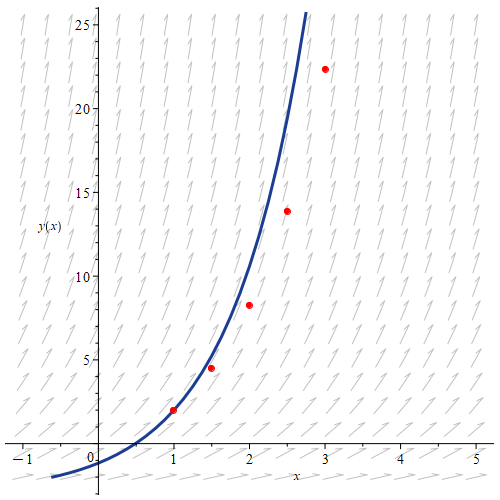
\includegraphics[width=0.6 \textwidth]{figur1.png}
\end{center}
Jo længere væk fra begyndelsesværdien vi kommer jo dårligere bliver punkterne estimeret. 
Hvis jeg derimod havde valgt \(h=0.1\) ville punkterne ligge noget tættere på den sande løsningskurve, men det ville samtidigt resultere i flere beregninger.

\end{document}